% Aspectratio 16:9 is the standard for modern projectors/monitors
\documentclass[aspectratio=169, 11pt]{beamer}

% Import my custom style
\usepackage{hcmus_beamer}

% Define image directory
\graphicspath{ {./images/} }

% --- PRESENTATION METADATA ---
%\titlegraphic{
%    \includegraphics[height=1.5cm]{hcmus_logo}
%}
\title[Multivariate Kernel Density Estimation]{Multivariate Kernel Density Estimation}

\subtitle{Computational Statistics Course Project}

% --- OPTIMIZED STANDARD METADATA ---

% 1. XỬ LÝ AUTHOR: Dùng Bảng (Tabular) để khóa vị trí
% Thay vì dùng \and, ta tạo 3 cột cứng cho 3 người.
\author[Group 3]{
    \small % Giảm cỡ chữ một chút để 3 tên dài không bị tràn lề
    \begin{tabular}{c c c} % 3 cột căn giữa (Center - Center - Center)
        \textbf{Khang Nguyen} & \textbf{Nhat Tien Nguyen} & \textbf{Phuc Loc Nguyen} \\
        \scriptsize \textit{25C01035} & \scriptsize \textit{25C01039} & \scriptsize \textit{25C01041}
    \end{tabular}
}

% 2. XỬ LÝ INSTITUTE: Căn giữa Logo và Tên trường
\institute[HCMUS]{
    \vspace{0.5em} % Tạo khoảng thở
    \begin{columns}[c] % Căn giữa theo chiều dọc
        % Logo (bên trái tâm)
        \begin{column}{0.4\textwidth}
            \flushright % Đẩy logo sát về phía chữ
            \includegraphics[height=1.6cm, keepaspectratio]{images/hcmus_logo}
        \end{column}

        % Tên trường (bên phải tâm)
        \begin{column}{0.6\textwidth}
            \flushleft % Đẩy chữ sát về phía logo
            \scriptsize Master of Data Science \\
            \small \textbf{University of Science, VNU-HCM}
        \end{column}
    \end{columns}
}

% 3. Ngày tháng
\date{\small \today}

\setbeamertemplate{navigation symbols}{} % Tắt icon điều hướng thừa thãi

% Tự định nghĩa lại footer: Chỉ hiện số trang/tổng số trang ở góc phải
\setbeamertemplate{footline}{
    \hbox{
        \begin{beamercolorbox}[wd=1\paperwidth, ht=2.25ex, dp=1ex, right]{}
            % Màu chữ xám nhạt cho đỡ chói
            \color{gray} \small \insertframenumber{} / \inserttotalframenumber \hspace*{2em}
        \end{beamercolorbox}
    }
    \vspace*{0.5em} % Tạo khoảng thở nhỏ ở đáy
}

% --- MAIN DOCUMENT ---
\begin{document}

% 1. Title Slide
\begin{frame}
    \titlepage
\end{frame}

% 2. Table of Contents
\begin{frame}{Outline}
    \tableofcontents[hideallsubsections] % Cleaner look
\end{frame}

% 3. Modular Content
% Each member works on their own file in the 'sections' folder
\section{Problem}


% --- SLIDE 1: Problem Statement ---
\begin{frame}{Problem Statement}
\begin{itemize}
    \item<1-> \textcolor{blue}{Kernel density estimation (KDE)} is a flexible nonparametric method.
    \item<2-> \textcolor{orange}{Univariate KDE} is well understood and easy to implement.
    \item<3-> In practice, data are often \textcolor{purple}{multivariate}.
    \item<4-> This motivates extending KDE to \textcolor{teal}{$p$-dimensional spaces}.
\end{itemize}
\end{frame}


% --- SLIDE 2: THE PROBLEM ---
\begin{frame}{The Curse of Dimensionality}
    \begin{columns}
        % Left Column: Concepts
        \begin{column}{0.5\textwidth}
            \begin{alertblock}{The Challenge}
                High-dimensional space ($p > 3$) is vastly different from univariate space.
                Data becomes incredibly \textbf{sparse}.
            \end{alertblock}

            \pause

            \vspace{1em}
            \textbf{Key Implications:}
            \begin{itemize}
                \item Points have very few near neighbors.
                \item ``Empty space'' phenomenon: For $p=10$, $>50\%$ of mass lies in the extreme tails ($>1.6\sigma$).
                \item Visualization is difficult without dimension reduction.
            \end{itemize}
        \end{column}

        % Right Column: Visual
        \begin{column}{0.5\textwidth}
            \centering
            \includegraphics[width=0.9\linewidth]{sparseness_highdim}

            \vspace{0.3em}
            \captionof{figure}{\scriptsize Sparseness in High Dimensions}
        \end{column}
    \end{columns}
\end{frame}

\subsection{General Multivariate Kernel Density Estimators}
% --- SLIDE 2: GENERAL FORMULA ---
\begin{frame}{General Multivariate Estimator}
    Let $\vect{x}$ be a $p$-dimensional random vector. The general estimator is defined as:

    \begin{block}{General Multivariate KDE}
        \begin{equation}
            \hat{f}(\vect{x}) = \frac{1}{n |\vect{H}|} \sum_{i=1}^{n} K\left( \vect{H}^{-1} (\vect{x} - \vect{x}_i) \right)
        \end{equation}
    \end{block}

    \vspace{1em}
    \textbf{Components:}
    \begin{itemize}
        \item $\vect{H}$ ($p \times p$): \textbf{Bandwidth Matrix} (controls orientation and scaling).
        \item $|\vect{H}|$: Determinant of $\vect{H}$ (normalizing constant).
        \item $K$: Multivariate kernel function (usually symmetric).
    \end{itemize}

    \vspace{0.5em}
    \small \textit{Note: Specifying a full matrix $\vect{H}$ is computationally expensive.}
\end{frame}
\section{Simplification by Product Kernel method}
% --- SLIDE 3: PRODUCT KERNELS (ANIMATED) ---
\begin{frame}{Practical Approach: Product Kernels}
    % 1. CONCEPT: Start with the core assumption
    To simplify the complexity, we assume \alert<2>{\textbf{independence}} between dimensions.
    \begin{itemize}
        \item This implies the Bandwidth Matrix $\vect{H}$ is \textbf{diagonal}.
    \end{itemize}

    % 2. FORMULA: Highlight the 'Product' operator to show simplification
    \begin{block}{The Product Estimator}
        \begin{equation}
            \hat{f}(\vect{x}) = \frac{1}{n} \sum_{i=1}^{n} \underbrace{\alert<3>{\prod_{j=1}^{p}} \frac{1}{\alert<4>{h_j}} K\left( \frac{x_j - X_{ij}}{\alert<4>{h_j}} \right)}_{\text{Product of univariate kernels}}
        \end{equation}
    \end{block}

    \vspace{0.5em}

    \begin{columns}[c]
        % Left Column: Advantages (Sequential Disclosure)
        \begin{column}{0.55\textwidth}
           \textbf{Key Advantages:}
           \begin{itemize}
               \setlength\itemsep{0.6em}

               % CLICK 4: Parameter Reduction (The biggest win)
               \item<4-> \textbf{Parameter Reduction:}
               \newline \footnotesize Reduces unknowns from \alert<4>{$O(p^2)$} (full matrix) to \alert<4>{$O(p)$} (vector).

               % CLICK 5: Efficiency
               \item<5-> \textbf{Computational Efficiency:}
               \newline \footnotesize No expensive matrix inversion needed.

               % CLICK 6: Flexibility
               \item<6-> \textbf{Flexibility:}
               \newline \footnotesize Allows distinct bandwidth $h_j$ for each dimension.
           \end{itemize}
        \end{column}

        % Right Column: Visual Consequence (Static or Revealed)
        % We keep it visible to show the "Constraint" of this method
        \begin{column}{0.45\textwidth}
            \centering
            % Use the specific image name you provided
            \includegraphics[width=0.9\linewidth, height=4.5cm, keepaspectratio]{2D_Contour_Density_Surface}
            \vspace{-0.2em}
            \captionof{figure}{\scriptsize Consequence: \alert<2>{Axis-aligned} Contours}
        \end{column}
    \end{columns}
\end{frame}
\section{Bandwidth Selection}
% --- SLIDE 4: BANDWIDTH SELECTION (ANIMATED) ---
\begin{frame}{Bandwidth Selection (Scott's Rule)}
    To minimize the error (AMISE), we select the bandwidth $h_j$ for each dimension:

    \vspace{1em}
    \begin{block}{Multivariate Scott's Rule}
        \begin{equation}
            h_j = \alert<2>{\hat{\sigma}_j} \left( \frac{4}{\alert<3>{n}(\alert<4>{p}+2)} \right)^{\frac{1}{\alert<4>{p}+4}}
        \end{equation}
    \end{block}

    \vspace{1em}
    \textbf{Interpretation:}
    \begin{itemize}
        \item<2-> \alert<2>{$\hat{\sigma}_j$}: The standard deviation (scale) of variable $j$.
        \item<3-> \alert<3>{$n$}: Sample size. More data $\to$ smaller bandwidth (finer detail).
        \item<4-> \alert<4>{$p$}: Number of dimensions.
        \begin{itemize}
            \item As $p \uparrow$, data becomes sparse.
            \item We need \textbf{wider bandwidths} to cover the gaps.
        \end{itemize}
    \end{itemize}
\end{frame}
\section{Radial Symmetry Kernel Asumnption}
% --- SLIDE 4.5: THE SPHERICAL ESTIMATOR (THE BRIDGE) ---
\begin{frame}{Alternative Simplification: Radial Symmetry}
    \small
    Instead of multiplying univariate kernels, what if we use a single \textbf{Radially Symmetric} kernel $K$ for the whole $p$-dimensional space?

    \vspace{0.5em}

    % 1. THE FORMULA (Equation 10.42)
    \begin{block}{The Spherical Estimator (Eq. 10.42)}
        We use a \textbf{single scalar bandwidth} $h$ for all dimensions:
        \begin{equation}
            \hat{f}(\vect{x}) = \frac{1}{n h^p} \sum_{i=1}^{n} K \left( \frac{\vect{x} - \vect{X}_i}{h} \right)
        \end{equation}
        {\footnotesize \textit{(Where $K$ depends only on the distance $||\vect{x} - \vect{X}_i||$, e.g., Multivariate Epanechnikov)}}
    \end{block}

    \vspace{0.5em}

    % 2. THE GEOMETRY & LIMITATION
    \begin{columns}[c]
        % Left: Characteristics
        \begin{column}{0.55\textwidth}
            \begin{itemize}
                \setlength\itemsep{0.8em}
                \item<2-> \textbf{Geometry:} The kernel shape is a perfect \textbf{Hyper-Sphere} (Ball).
                \item<3-> \textbf{Simplicity:} Only 1 parameter ($h$) to tune!
                \item<4-> \textbf{\textcolor{red}{The Catch:}} It assumes data spreads \textbf{equally} in all directions.
            \end{itemize}
        \end{column}

        % Right: Visual Mismatch
        \begin{column}{0.45\textwidth}
            \centering
            \onslide<4->{
                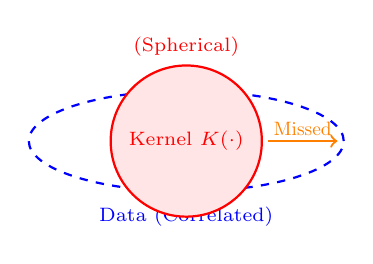
\begin{tikzpicture}[scale=0.8]
                    % Data distribution (Ellipse)
                    \draw[thick, dashed, blue] (0,0) ellipse (2.5cm and 0.8cm);
                    \node[blue] at (0, -1.2) {\scriptsize Data (Correlated)};

                    % Kernel (Circle) - Trying to fit
                    \draw[thick, red, fill=red!10] (0,0) circle (1.2cm);
                    \node[red] at (0, 0) {\scriptsize Kernel $K(\cdot)$};
                    \node[red] at (0, 1.5) {\scriptsize (Spherical)};

                    % Arrows indicating mismatch
                    \draw[->, orange, thick] (1.3,0) -- (2.4,0);
                    \node[orange, scale=0.7] at (1.85, 0.2) {Missed};
                \end{tikzpicture}

                \vspace{0.5em}
                \footnotesize \textcolor{red}{Problem:} A sphere fits poorly inside a long ellipse.
            }
        \end{column}
    \end{columns}

    % 3. TRANSITION TO WHITENING
    \vspace{1em}
    \centering
    \onslide<5->{
        \textbf{Idea:} \textit{If the Kernel can't stretch to fit the Data, why don't we \textbf{shrink the Data} to fit the Kernel?} \\
        \Large $\Downarrow$ \\
        \normalsize \textbf{Next Step: Whitening}
    }
\end{frame}
\section{Decorrelation by Whiteninig}


% --- SLIDE 6: THE TRANSFORMATION WORKFLOW (ANIMATED) ---
\begin{frame}{Implementation Workflow (Step-by-Step)}
    \begin{columns}[c]
        % Left Column: The Steps (Text)
        \begin{column}{0.55\textwidth}
            \small
            \textbf{Standard Operating Procedure (SOP):}

            % [<+->] automatically uncovers items one by one (1, then 2, then 3...)
            \begin{enumerate}[<+->]
                \setlength\itemsep{0.5em}

                \item \textbf{Decompose:} Compute Eigen-decomposition of Covariance Matrix $\hat{\vect{\Sigma}} = \vect{P} \vect{\Lambda} \vect{P}^T$.

                \item \textbf{Transform (Whitening):} Rotate data to eliminate correlation.
                % The box appears with item 2
                \begin{equation*}
                    \boxed{\vect{Z}_i = \vect{\Lambda}^{-1/2}\vect{P}^T(\vect{x}_i - \bar{\vect{x}})}
                \end{equation*}

                \item \textbf{Estimate:} Apply simple Product Kernel on the whitened data $\vect{Z}$.

                \item \textbf{Reconstruct:} Adjust density scale to original space (Jacobian determinant).
                \[ \hat{f}_{\vect{X}}(\vect{x}) = \hat{f}_{\vect{Z}}(\vect{z}) \cdot \alert{|\hat{\vect{\Sigma}}|^{-1/2}} \]
            \end{enumerate}
        \end{column}

        % Right Column: The Image (Static)
        % We keep the image visible from the start so they can reference it while reading steps
        \begin{column}{0.45\textwidth}
            \centering
            \includegraphics[width=0.95\linewidth, height=6cm, keepaspectratio]{whitening_transform}
            \vspace{0.2em}
            \captionof{figure}{\scriptsize $\vect{X}$ (Correlated) $\to$ $\vect{Z}$ (Spherical)}
        \end{column}
    \end{columns}
\end{frame}

% --- SLIDE 7: PERFORMANCE COMPARISON (ANIMATED) ---
\begin{frame}{Performance Comparison}

    \begin{columns}[c]
        % Left Column: Image (Always visible to set the context)
        \begin{column}{0.6\textwidth}
            \centering
            \includegraphics[height=4.0cm, keepaspectratio]{white_mkde_vs_native}
            \vspace{-0.2em}
            \captionof{figure}{\scriptsize Naive (Left) vs. Whitened (Right)}
        \end{column}

        % Right Column: Text Observations (Revealed sequentially)
        \begin{column}{0.4\textwidth}
            \small
            \textbf{Key Observations:}
            \begin{itemize}
                \setlength\itemsep{0.5em}

                % Click 2: Reveal the Failure analysis
                \item<2-> \textbf{Naive Approach:}
                \textcolor{red}{\textbf{Fail.}} Constrained to axis-aligned shapes. Misses diagonal correlations.

                % Click 3: Reveal the Success analysis
                \item<3-> \textbf{Whitened MKDE:}
                \textcolor{darkgreen}{\textbf{Success.}} Contours adapt perfectly to the data's orientation.
            \end{itemize}
        \end{column}
    \end{columns}

    \vspace{1em}

    % Click 4: Reveal the Final Verdict (The "Takeaway" message)
    \onslide<4->{
        \begin{alertblock}{Final Verdict}
            \centering \footnotesize
            Whitening enables \textbf{Product Kernels} to model complex correlations with $O(n)$ efficiency.
        \end{alertblock}
    }
\end{frame}


% --- SLIDE 5: THE MATHEMATICAL SHORTCUT (ANIMATED) ---
\begin{frame}{Generalized Estimator (Theory)}
    Instead of performing manual transformation steps, we can mathematically express the estimator directly using the **Mahalanobis Distance**:

    % 1. The Equation is always visible, but parts light up sequentially
    \begin{block}{General Multivariate KDE Equation (10.44)}
        \begin{equation}
             \hat{f}(\vect{x}) = \frac{\alert<2>{|\hat{\vect{\Sigma}}|^{-1/2}}}{nh^p} \sum_{i=1}^{n} K \left( \frac{\alert<3>{(\vect{x} - \vect{X}_i)^T \hat{\vect{\Sigma}}^{-1} (\vect{x} - \vect{X}_i)}}{h} \right)
        \end{equation}
    \end{block}

    \vspace{1em}
    % 2. Columns appear strictly when their corresponding math term is highlighted
    \begin{columns}[t]
        % Left Column: Appears on Click 2 (Matches |\Sigma|^{-1/2})
        \begin{column}{0.48\textwidth}
            \onslide<2->{
                \textbf{\alert<2>{1. Volume Correction:}}
                \begin{itemize}
                    \item The term $|\hat{\vect{\Sigma}}|^{-1/2}$ adjusts the density scale.
                    \item Ensures the total probability integrates to 1 after "stretching" space.
                \end{itemize}
            }
        \end{column}

        % Right Column: Appears on Click 3 (Matches Mahalanobis Distance)
        \begin{column}{0.48\textwidth}
            \onslide<3->{
                \textbf{\alert<3>{2. Shape Adaptation:}}
                \begin{itemize}
                    \item Uses \textbf{Mahalanobis Distance} instead of Euclidean.
                    \item Captures the correlation structure (orientation) of the data.
                \end{itemize}
            }
        \end{column}
    \end{columns}
\end{frame}
% --- APPENDIX: FOURIER KDE ---
\appendix % Đánh dấu bắt đầu phụ lục (Reset số trang hoặc đổi màu)

% --- SLIDE A1: THE THEORETICAL FOUNDATION ---
\begin{frame}{Appendix A: Beyond Gaussian (Fourier Approach)}
    \small
    \textbf{Motivation:} Standard KDE struggles with bandwidth matrices ($\mathbf{H}$) in high dimensions. Is there a better way?

    \vspace{0.5em}
    \begin{block}{The Fourier Integral Theorem (Identity)}
        Any square-integrable function $f(\vect{x})$ can be reconstructed \textbf{exactly} via:
        \begin{equation}
            f(\vect{x}) = \lim_{R \to \infty} \frac{1}{\pi^d} \int_{\mathbb{R}^d} \prod_{j=1}^{d} \frac{\sin(R(x_j - t_j))}{x_j - t_j} f(\vect{t}) d\vect{t}
        \end{equation}
    \end{block}

    \vspace{0.5em}
    \begin{columns}[c]
        \begin{column}{0.6\textwidth}
            \textbf{The Estimator (Monte Carlo approx):}
            $$ \hat{f}_{n,R}(\vect{x}) = \frac{1}{n \pi^d} \sum_{i=1}^{n} \prod_{j=1}^{d} \underbrace{\frac{\sin(R(x_j - X_{ij}))}{x_j - X_{ij}}}_{\text{Sinc Kernel}} $$
        \end{column}
        \begin{column}{0.4\textwidth}
            \begin{alertblock}{Key Difference}
                \centering \footnotesize
                It uses the \textbf{Sinc Kernel} instead of Gaussian.
                \\ $\text{sinc}(u) = \frac{\sin(u)}{u}$
            \end{alertblock}
        \end{column}
    \end{columns}
\end{frame}

% --- SLIDE A2: THE "KILLER FEATURE" (AUTOMATIC DEPENDENCE) ---
\begin{frame}{Appendix B: The "Magic" of Fourier KDE}
    \textbf{The Big Question:} How does it handle correlation without a matrix $\mathbf{H}$?

    \vspace{1em}
    \begin{columns}[T]
        % --- LEFT: GAUSSIAN STRUGGLE ---
        \begin{column}{0.48\textwidth}
            \begin{block}{1. Gaussian KDE (Traditional)}
                \small
                To capture correlation, we \textbf{MUST} estimate a full matrix $\mathbf{H}$ (or $\mathbf{\Sigma}^{-1}$).
                \vspace{0.5em}
                \begin{itemize}
                    \item $\prod K(x_j)$ (Diagonal) $\to$ \textcolor{red}{Fails (Axis-aligned)}.
                    \item Full $\mathbf{H}$ $\to$ \textcolor{orange}{Expensive ($O(d^2)$)}.
                \end{itemize}
            \end{block}
        \end{column}

        % --- RIGHT: FOURIER MAGIC ---
        \begin{column}{0.48\textwidth}
            \onslide<2->{
                \begin{alertblock}{2. Fourier KDE (Advanced)}
                    \small
                    \textbf{Theorem:} A simple product of 1D Sinc kernels \textbf{automatically} recovers the joint density structure.
                    \vspace{0.5em}
                    \begin{itemize}
                        \item \textbf{No Matrix needed!} Just a scalar $R$.
                        \item Captures rotation/correlation natively via the Fourier domain.
                    \end{itemize}
                \end{alertblock}
            }
        \end{column}
    \end{columns}

    \vspace{1em}
    \centering
    \onslide<3->{
        \textbf{\textcolor{darkred}{Verdict:}} Fourier KDE bypasses the "Bandwidth Matrix Selection" headache entirely.
    }
\end{frame}

% --- SLIDE A3: PERFORMANCE & CONVERGENCE ---
\begin{frame}{Appendix C: Performance Superiority}
    \small
    Why should we care? Because it converges faster.

    \vspace{1em}
    \begin{columns}[c]
        \begin{column}{0.5\textwidth}
            \textbf{Convergence Rate (MISE):}
            \vspace{0.5em}
            \begin{itemize}
                \setlength\itemsep{1em}
                \item \textbf{Standard KDE:}
                $$ O(n^{-4/(4+d)}) $$
                \textit{(Suffer from Curse of Dimensionality)}

                \item \textbf{Fourier KDE (Supersmooth):}
                $$ \alert{O(n^{-1} (\log n)^k)} $$
                \textit{(Almost parametric rate $1/n$!)}
            \end{itemize}
        \end{column}

        \begin{column}{0.5\textwidth}
            \centering
            % Vẽ minh họa tốc độ hội tụ đơn giản
            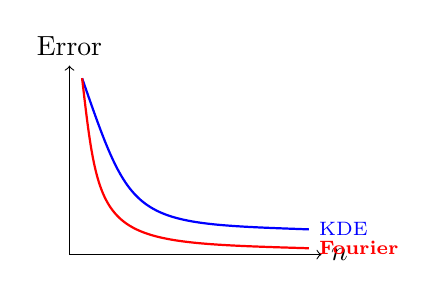
\begin{tikzpicture}[scale=0.8]
                \draw[->] (0,0) -- (4,0) node[right] {$n$};
                \draw[->] (0,0) -- (0,3) node[above] {Error};
                \draw[thick, blue] (0.2, 2.8) .. controls (1, 0.5) .. (3.8, 0.4) node[right] {\scriptsize KDE};
                \draw[thick, red] (0.2, 2.8) .. controls (0.5, 0.2) .. (3.8, 0.1) node[right] {\scriptsize \textbf{Fourier}};
            \end{tikzpicture}
            \vspace{0.5em}
            \captionof{figure}{\scriptsize Faster error decay}
        \end{column}
    \end{columns}

    \vspace{1em}
    \footnotesize
    \textit{Source: Ho, N., \& Walker, S. G. (2021). Multivariate Smoothing via the Fourier Integral Theorem.}
\end{frame}
% --- FINAL SLIDE: Q&A & CONTACT ---
\begin{frame}[plain] % [plain] để xóa số trang và header, tạo sự tập trung
    \centering

    % 1. Lời cảm ơn trang trọng (Standard Formal Phrase)
    \vspace{1cm}
    {\Huge \bfseries \textcolor{darkred}{Thank You for Your Attention!}}

    \vspace{1.5cm}

    % 2. Phần Q&A
    {\LARGE \textbf{Q \& A}} \\
    \vspace{0.5em}
    \textit{\color{gray} We are open to any questions or feedback.}

    \vspace{2cm}

    % 3. Thông tin kết nối (Project Resource) - Dấu hiệu của Senior
    % Dùng box bo tròn để chứa link GitHub/Email
    \begin{beamercolorbox}[sep=8pt,center,shadow=true,rounded=true]{block title}
        \textbf{Project Source Code \& Slides:} \\
        \vspace{0.3em}
        \footnotesize \url{https://github.com/khang3004/Multivariate_KernelDensity_Estimators.git}
    \end{beamercolorbox}

    \vspace{0.5em}
    \scriptsize \textbf{Contact:} \texttt{21C0103580@student.hcmus.edu.vn}

\end{frame}
\end{document}